\chapter{Pulse Microstructure}
\label{chapter:microstructure}
\chaptermark{Microstructure}

% \textbf{Think this is the largest set of B0329+54 single pulses 
% studied at $\mu$s. Check. \\ 
% Maybe include gamma arguments P/tms about 1000 for this pulsar 
% seems to be too big for flux tubes \\ 
% bartel \citep{1981A&A....93...85B} observed with 2.5 $\mu s$}

% ================================================================================
% CHAPTER OVERVIEW
% ================================================================================

\section{Chapter Overview}
In this chapter we present results from full-polarization  
single-pulse observations of pulsar B0329+54. 
We have over $10^4$ pulses 
collected with the Algonquin Radio Observatory 46\,m telescope
with 2.56\,$\mu$s time resolution and 390\,kHz 
frequency bins. 
We find microstructure to be a generic broad-band property of 
individual pulses at 400-800\,MHz.
We also analyze B0329+54's quasi-periodic structure
using a reduced autocorrelation function (rACF). 
Unlike in other pulsars, 
we do not find a characteristic timescale in its quasi-periodicity, 
although the range of of periods is consistent with the known
$t_{\mu} \approx 6 \times 10^{-4} P$ and 
$T_{\mu} \approx 10^{-3} P$ relations. 
Our polarimetry results agree with 
\citet{2015ApJ...806..236M}, in that the periodicity 
of both linear and circular polarization microstructure 
traces closely the total power. 
% This is difficult to 
% accommodate in the model where microbursts represent 
% single charge bunches emitting curvature radiation 
% in vacua. 
We also investigate the spectral properties 
of micropulses within a sub-pulse. It is shown that the microstructure not 
only has a wide bandwidth, but that adjacent broad-band 
microstructures can have very different spectra. 

%================================================================================
% INTRODUCTION
% ================================================================================

\section{Introduction}

Within only a few years of the discovery of pulsar B1919+21
in 1967 it had 
become clear that there was great variation between 
individual pulses, and 
even structure within pulses 
\citep{1968Natur.218.1122C, 1975ApJ...196...83M, 1975Natur.257..293R}. 
% Insert citation for this variation.
Each pulsar's folded and integrated profile 
is highly reproducible and specific to that pulsar, 
however the pulses of which they are comprised are 
diverse in a multitude of ways \citep{1998pulsarastronomy}. 
Variation of polarization fraction and mode, intensity 
fluctuations of sub-pulses, and variable arrival times 
are examples of the pulse-to-pulse dynamics. Nulling 
and pulse drifting are also common, and still these 
ostensibly stochastic phenomena result in recognizable 
folded profiles. An example of this is shown in 
Fig.~\ref{fig-pulse_outline}, in data taken at ARO. 

\begin{figure}[!h]
\begin{center}
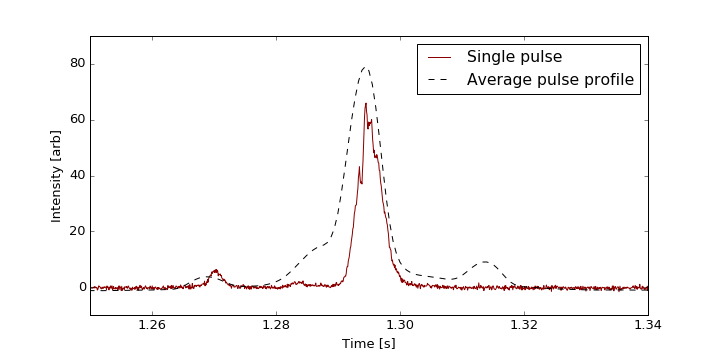
\includegraphics[trim={0in 0in 0in 0in}, width=1\textwidth]{./figures/microstructure/B0329_average_single.png}
\vspace{0.0cm}
\caption{The average profile of pulsar B0329+54 (dashed, black line)
plotted over a single pulse (solid, maroon line). Though 
there is significant variation from pulse to pulse in 
each of the sub-components (of which there are 
as many as 9 \citep{2001ApJ...555...31G}), 
the average profile is 
well known and repeatable. It can be thought of as a 
probability distribution from which the power in each 
phase bin for a single pulse is drawn.}  
\vspace{-0.4cm}   
\label{fig-pulse_outline}
\end{center}
\end{figure}

Understanding the physical mechanism by which pulsars emit in the 
radio has proven one of the hardest problems 
in modern astrophysics \citep{1975ARA&A..13..511G, 2000ASPC..202..721M}. 
Most of what is known has come 
from folded pulse profiles, but given the substantial 
phenomenology on timescales of individual pulses, there 
is good reason to study them.

On the shortest timescales, microstructure appears in a number of pulsars 
\citep{1975PhDT.........9C, 1982ApJ...254L..35B, 
1998A&A...332..111L, 2002A&A...396..171P}. 
This usually involves 
intensity variation on sub-millisecond timescales. 
They can exhibit periodic oscillatory fluctuations 
as well as broad-band features \citep{1981A&A....93...85B}. 
%\textbf{DESCRIBE IN MORE DETAIL}
Although the phenomenon has been seen in a number of slow pulsars 
at a range of frequencies, there is 
no agreed upon explanation for the origin of microstructure 
\citep{1998A&A...332..111L}. 
\citet{vanhorn} argued the phenomenon was not magnetospheric
but rather a result of neutron star vibrations, 
hence the periodic nature of the substructure. 
Another explanation has been to evoke propagation 
effects in the pulsar magnetosphere. Most commonly, though, 
models for these $\sim$microsecond intensity 
fluctuations have assumed it is fundamentally 
related to the emission mechanism 
rather than a separate process occurring elsewhere 
in the magnetosphere \citep{1998A&A...332..111L}.

Before linking microstructure to broader emission mechanisms, 
it is useful to remind ourselves about the potential 
sources of radio emission in pulsars. 
One prominent explanation is the vacuum curvature 
radiation model. Curvature radiation is similar to 
synchrotron except with a pitch angle that is nearly zero.
In the pulsar magnetosphere, this happens when electrons or positrons 
travel along the very strong curved
magnetic field lines, radiating 
at some critical frequency $\nu_c \sim \gamma^3 c/r_B$, 
where $r_B$ is the radius of curvature of the field lines and 
$\gamma$ is the Lorentz factor
\citep{1998pulsarastronomy}. Given the 
expected relativistic electron-positron plasma over-density at the
pulsar's polar caps and the strong magnetic fields there, 
curvature radiation seems like a natural explanation 
for radio emission. One difficulty with the model is that 
due to the exceedingly high brightness temperatures of 
pulsars, it has always been known that 
coherent emission is needed. For the vacuum curvature 
scenario, this requires ``charged bunches" of electrons 
($\sim$10$^{15}$ particles) emitting coherent curvature radiation 
\citep{2004ApJ...600..872G}, and it is not obvious 
how these bunches would be created.

The single-particle vacuum curvature-radiation model 
can be informed by observations microstructure and 
its polarization. Since the sub-pulses that make 
up individual pulses can be further broken down into 
microstructures, those microbursts should show phenomena 
predicted by thoery. The consequences of 
an incoherent sum of charged bunches 
emitting coherent curvature radiation can be found 
in \citet{1990A&A...234..269G} and summarized 
in \citet{2015ApJ...806..236M}.

Few detailed polarization studies of 
microstructure have been carried out. 
\citet{1978A&A....64...27F} commented on the qualitative 
polarization properties of microstructure seen in B1133+16. 
\citet{2002MNRAS.334..523K} quantitatively analyzed polarimetry 
observations of Vela's microstructure. Recently, however, 
\citet{2015ApJ...806..236M} made a convincing case for 
studying short-timescale 
fluctuations of polarized pulsar emission. 
They observed almost three 
dozen sources with $\sim$60\,$\mu$s time-resolution at 
Arecibo with periods ranging from 0.15-3.7 seconds.



% ================================================================================
% THEORY AND IMPLEMENTATION
% ================================================================================

\section{B0329+54 Individual Pulses}

\subsection{Observations}

The data for our B0329+54 single-pulse analysis 
were taken at the Algonquin Radio Observatory (ARO). 
The refurbished 46\,m antenna was mounted with a 400-800\,MHz 
CHIME four-leaf clover feed, the details 
of which are described in Chapter \ref{chapter:chime}. 
We attached to it a custom back-end 
made from CHIME hardware and software that can write voltage 
data to disk with $\sim$390\,kHz spectral resolution 
and 2.56\,$\mu$s temporal resolution. We refer to this as ``baseband". 
Though the data is channelized with a polyphase filter bank (PFB),
the process is invertible and we are able to 
de-channelize in order to coherently dedisperse offline. Data are written 
in the VDIF specification, similar to the Pathfinder data format 
described in Chapter \ref{chapter:beamforming}. However in 
the case of ARO, since we have 2 channels instead of 256, we do 
not need 16 FPGA boards and 16 GPU nodes to process the data. 
Therefore frequencies need not be reassembled because 
each frame contains all 1024 contiguous frequencies. There 
are also slight changes to the header. 
We observed the pulsar for roughly 2 hours on 1 August 
2014, for more than 10$^4$ pulses. 


\subsection{Data post-processing}
\label{sec-b0329analysis}

We use a VLBI pulsar analysis code-base called 
{\tt scintellometry}, which was built for 
correlating baseband data from different telescopes 
with differing data formats\footnote{https://github.com/mhvk/scintellometry}. 
Though the code is able to coherently dedisperse, 
B0329+54 is slow and has a DM of only 
$\sim$27 pc cm$^{-3}$, and we have found it is sufficient to do ``by-channel" 
dedispersion. This means stepping through each frequency 
of the channelized voltage data, inverse Fourier transforming 
that frequency's time series, and dedispersing that up-channelized 
chunk. The resultant DM-smearing in the case of 
B0329+54 is negligible. 

The two dedispersed voltage time-streams are then correlated, 
providing four real numbers per time and frequency. 
Out of these correlations the Stokes parameters 
can be constructed. The four numbers are an autocorrelation for each 
polarization, and the real and imaginary components of the
cross-correlation. The output array is therefore,

\begin{equation}
D = \begin{pmatrix}
\left< X_0X_0^*\right> & \left< \Re e\{X_0X_1^*\}\right >\\ 
 \left< \Im m\{X_0X_1^*\}\right > & \left< X_1X_1^*\right>
\end{pmatrix}.
\end{equation}
\\
\noindent By rearranging these, the Stokes parameters can 
be obtained as follows,
\\
\begin{equation}
\begin{pmatrix}
\left< X_0X_0^*\right> & \left< X_0X_1^*\right >\\ 
 \left< X_0^*X_1 \right > & \left< X_1X_1^*\right>
\end{pmatrix} = 
\begin{pmatrix}
I + Q & U + iV\\ 
U -iV & I - Q
\end{pmatrix}.
\end{equation}


\noindent These intensities are either folded 
or written to a dedispersed time and frequency {\tt numpy} 
array with arbitrary time rebinning. 

Before the polarization data can be analyzed, 
we must remove two effects. The first is the 
sinusoidal phase in frequency introduced by cable delays. 
This comes from that fact that the two polarizations signals, 
$X_0$ and $X_1$, end up with slightly different instrumental 
phases due to things like disparate cable lengths. When 
the signals are correlated, a constant phase offset (time lag) 
becomes a sinusoidal oscillation in frequency. 
Written in terms of the Stokes parameters
this transformation takes,

\begin{equation}
X_0 X_1^* = U + iV,
\end{equation}

\noindent and makes the cross-pol correlation

\begin{equation}
X_0 X_1^* \rightarrow \left (U + iV \right) \times e^{2\pi i \nu \tau},
\end{equation}

\noindent where $\tau$ is the instrumental time lag
between the two polarizations. This rotates Stokes V 
into Stokes U, thereby leaking circular into linear polarization.

Another effect is Faraday rotation, which is significant 
for B0329+54 in our band. Its RM is $\sim$64\,rad\,m$^{-2}$, 
resulting in several phase wraps between 400-800\,MHz.
Unlike cable delays, the Faraday effect rotates the 
linear polarization vector, $P_L$, defined by:

\begin{equation}
P_L \equiv Q + iU.
\end{equation}

\noindent Similar to dispersion, it depends on $\lambda^2$.
The linear polarization is rotated as,

\begin{equation}
P_L \rightarrow P_L\, e^{2i\, \textrm{RM} \, \lambda^2}.
\end{equation}

We remove these two effects by doing a joint fit 
of the folded pulse profile at each frequency. We fit 
for time lag, $\tau$, $\rm RM$, Stokes 
Q, U, and V, as well as global phase offset, $\phi_{X_0,X_1}$. 
Though we do not do a full polarization calibration of 
the ARO feed, we have verified that its leakage is 
not too severe. This was done by measuring pulsar 
B1929+10, whose polarization angle swings by $\sim$80 
degrees in a known way, and comparing our results to a
calibrated template in the literature. We found 
only small deviations from the known template.

\section{Microstructure}

The polarization and 
total intensity of B0329+54 vary on a range of scales. 
Though the polarization in its folded profile is less than 
10$\%$ for both linear and circular, the 
mode and fraction from individual pulses 
jumps around. The pol-fraction for single pulses 
can surpass $70\%$. The total intensity is modulated 
at a number of different locations.
In the ISM, scintillation causes the pulsar's brightness to fluctuate 
on timescales of 5-30 minutes. Between individual pulses there is  
variation by factors of a few, which is presumably intrinsic 
to the source. Within a pulse (timescales $\lesssim 50$\,ms), 
brightness changes exist due to the multi-component nature 
of B0329's pulse profile. Finally, 
we see sub-millisecond fluctuations within these sub-pulses, 
which are the subject of this chapter.
Fig.~\ref{fig-alltscales} shows such variation on 
minutes, seconds, and millisecond timescales respectively,
going from top to bottom.

\begin{figure}[!h]
\begin{center}
\includegraphics[trim={1.5in 0in 1.5in 0in}, width=\textwidth]{./figures/microstructure/allscales.jpeg}
\caption{Pulsar B0329+54 intensity fluctuations 
on three different timescales. From top to bottom panel: roughly 
2,500 pulses over a half hour; pulse-to-pulse brightness 
variation; and intra-pulse variation on timescales of 50\,$\mu$s-10\,ms.}
\vspace{-0.75cm}   
\label{fig-alltscales}
\end{center}
\end{figure} 

\subsection{Quasi-periodicity}

Several pulsars are known to exhibit quasi-periodic 
trains of micropulses. \citet{1990AJ....100.1882C} 
found periodic variation in pulsars 0809+74, 0950+08, 
1133+16, 1944+17, and 2016+28. They found that each 
source's microstructure had a characteristic quasi-period, 
and that for some pulsars the strength of microstructure 
scaled inversely with frequency. 

In B0950+08, the periodic microstructure 
looks similar to Crab ``nanoshots".
The flux between micropulses almost entirely disappears 
and the bursts themselves are incredibly narrow ($\lesssim$10\,$\mu$s)
\citep{2002ARep...46..206P}. 
In B0329+54 we see quasi-periodic structures in a 
number of our strong pulses. However unlike in B0950 or 
the Crab, it seems to be a component that sits on 
top of an underlying smooth profile. To determine the 
timescales of this quasi-periodicity, we compute 
a reduced autocorrelation function (rACF). ACFs
have long been used to study microstructure
\citep[see][]{1978AZh....55.1024K, 1998A&A...332..111L}. 
It is computed as,

\begin{equation}
A(\tau) \equiv \frac{\int S(t)S(t + \tau) \, \textrm{d}t}{\int S^2(t)
\, \textrm{d}t},
\end{equation}

\noindent where $S(t)$ is any time-stream intensity, 
whether Stokes I, Q, U, or V. 
The maxima, minima, and slope changes of $A(\tau)$ 
can inform us about relevant timescales in the pulse
\citep{2015ApJ...806..236M}. 

For pulsars like B0329+54 whose microstructure often 
sits on top of a smoother pulse profile, $A(\tau)$
does not exhibit obvious structure. To avoid this problem 
we fit each sub-pulse with a Gaussian, subtract 
that off, then calculate the ``reduced" ACF using,

\begin{equation}
S'(t) \rightarrow S(t) - \mathcal{N}(\mu_{\rm fit}, \sigma^2_{\rm fit}).
\end{equation}


\begin{figure}[!h]
\vspace{-0.1cm}
\begin{center}
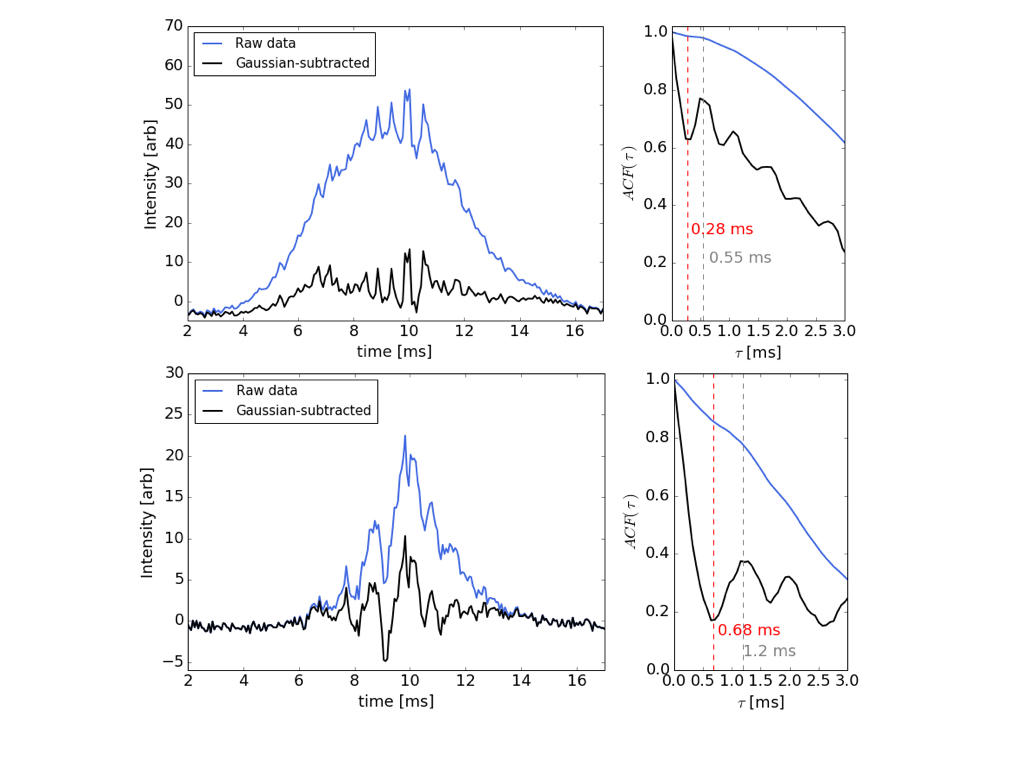
\includegraphics[trim={2in 1in 2in 0in}, width=\textwidth]{./figures/microstructure/quasi_periodicity.jpeg}
\caption{Periodicity and quasi-periodicity seen in 
     microstructure from 
     two different B0329+54 pulses, but on the same sub-pulse. 
     The top left panel shows a pulse with a periodic train of microbursts
     for both the raw profile (slate blue) and the 
     Gaussian-subtracted profile (black). The bottom 
     left panel shows broader and more moduluated 
     quasi-periodic microstructure. The right panels 
     show the corresponding ACF (slate blue) and rACF (black). 
     There are two striking features about these plots. The first 
     is that unlike other pulsars that exhibit microstructure,
     B0329+54 does not seem to have a characteristic period or width 
     to its structure. This is seen by comparing the first 
     minima and maxima of the correlation functions and 
     noticing they are at different timescales for the two 
     pulses. The second 
     is that the correlation function contains very little 
     information if a smooth component is not first subtracted, i.e., if 
     the rACF is not computed.}
\label{fig-quasistruct}
\end{center}
\end{figure}


An example of this is 
shown in the Fig.~\ref{fig-quasistruct}. The left 
panels shows bright single pulses with a
trains of microbursts for both $S(t)$ and $S'(t)$.
The right panel shows the corresponding ACFs. The 
black curve is the rACF, since it is 
the autocorrelation of a Gaussian-subtracted pulse. 

There is a known correlation between microstructure 
timescales and the pulsar period. 
\citet{2002MNRAS.334..523K} have shown the scaling to be,

\begin{equation}
t_\mu \approx 6\times10^{-4} P,
\end{equation}

\noindent where $P$ is the pulsar's period and 
$t_\mu$ is the timescale of individual microbursts, 
often estimated by the first local minimum in the ACF. 
This was consistent with the original claim by 
\citet{1979ApJ...233..981C}. 
\citet{2015ApJ...806..236M} used 24 L-band pulsars 
to revisit the relationship. Instead of using $t_\mu$, 
they used the period of quasi-periodic microstructure, 
$T_\mu$, and found it too increased 
with pulsar period as $\sim 10^{-3} P$. Here we will follow suit and 
focus primarily on the first local maximum. The reason we use
this rather than widths of individual microbursts 
is because those are often unresolved in time or scattered 
by the ISM. 

For B0329+54 we find the absence of a characteristic 
timescale, but consistency with 
the known $t_\mu-$ and $T_\mu-P$ relation. 
In Fig.~\ref{fig-quasistruct} we show 
an illustrative example of the differences in 
microstructure timescales from pulse to pulse. The 
top row's pulse has $t_\mu \sim 0.28$\,ms and 
$T_\mu \sim 0.55$\,ms, whereas the bottom row's pulse 
has $t_\mu \sim 0.68$\,ms and $T_\mu \sim 1.2$\,ms.
For B0329+54 we expect the first minima of rACFs
to be around $400$\,$\mu$s and the first maxima 
to be at $700$\,$\mu$s. In general, we find a range of 
$t_\mu \sim 100-1000$\,$\mu$s and 
$T_\mu \sim 500-2000$\,$\mu$s, which are consistent 
with the trend seen in other pulsars. 

There are two basic ways to get sub-millisecond 
variations in pulsars: angular beaming in the 
direction transverse to the observer, and actual temporal 
modulation in the magnetosphere.  
To interpret our measured timescales, we can start 
in the framework of a beaming model, in which 
the width of a micropulse is given by a 
radiating point source with some Lorentz factor, $\gamma$.
If we take $t_\mu$ as an upper limit for the 
width of a microburst, the pulse's width in radians is 
at most,

\begin{equation}
\phi = 2 \pi \, t_\mu / P\,.
\end{equation}

\noindent The Lorentz factor will be given by,

\begin{equation}
\gamma = \frac{1}{\phi\, \textrm{sin}\delta}\,,
\end{equation}

\noindent where $\delta$ is the angle between 
the pulsar's rotation axis and the line of site \citep{1998A&A...332..111L}.
Our results give a lower-limit on $\gamma$ of 
$\sim$500-1200. This is difficult to reconcile 
with several theoretical studies, which suggest 
the particles producing microstructure should have
$\gamma<100$ \citep{1992msem.coll..322A, 1998A&A...332..111L}.

In the temporal modulation picture, the effect
is not geometric but due to fluctuations in 
the intensity of waves propagating in the magnetosphere.
\citet{1983Ap&SS..97....9C} is an example of a temporal model, which 
does not require any beaming. In it, non-linear effects 
in the polar-cap plasma lead to intensity modulation 
along the radial direction.

\subsubsection{Polarized periodicity}

\citet{2015ApJ...806..236M} found that not only did 
their set of low-Galactic latitude pulsars 
have characteristic periodicities ($T_\mu$), but that 
those timescales were common across all Stokes 
parameters. Though we do not find a repeatable 
timescale in B0329+54, we do find its 
quasi-periodic microstructure to have the same 
timescales in Stokes I, V, and linear polarization.
We can see this visually 
for I and $|P_L|$ in Fig.~\ref{fig-polwaterfall}.

\citet{2015ApJ...806..236M} suggest that the similarity of 
the microstructure in 
linear and circular polarization with total intensity 
means the structures cannot be 
caused by coherent curvature radiation. 
\citet{1990A&A...234..269G} worked through the 
polarization consequences of an emission model 
in which the incoherent superposition of a large 
collection of sub-nanosecond pulses produced 
by the curvature mechanism.
They found the charged bunches in vacua predicts
sign-changing circular polarization. Since 
\citet{2015ApJ...806..236M} do not see 
handedness switching in individual microbursts, they conclude 
that such a mechanism cannot be the source of microstructure.  
We looked for a similar effect. In sub-pulses that had both significant 
Stokes V and modulated microstructure we did not find any sign-changes, 
even when the circular polarization went from right- to left-handed
across the sub-pulse. A caveat is that we do not find any 
microstructure as heavily modulated or resolved as the pulses 
\citet{2015ApJ...806..236M} found, meaning the microbursts 
we observe could be de-polarized or the sum of multiple 
modes. Therefore we do not claim that the 
absence of a sign change in B0329+54's microstructure 
can definitively rule out charged bunches emitting 
curvature radiation as their source. Instead we simply note 
that this feature was not seen, and might have been seen 
in the coherent curvature radiation model.





\begin{figure}[!h]
\vspace{-0.1cm}
\begin{center}
\includegraphics[trim={0in 0in 0in 0in}, width=\textwidth]{./figures/microstructure/micro_pol_waterfall.png}
\caption{An example of the way the linear polarization 
     traces periodic microstructure.}
\label{fig-polwaterfall}
\end{center}
\end{figure}

\subsection{Microburst spectral variation}

In some of the brightest pulses we find frequency 
variation between individual microbursts. Given 
the timescales invovled (200-1500\,$\mu$s), such 
variation is not expected to be due to propagation 
effects like scintillation. The top right panel of 
Fig.~\ref{fig-spectralvar} shows the same pulse at 
450\,MHz (red) and 640\,MHz (black). We isolate the
three brightest individual micropulses shaded by 
light blue, light red, and grey. One can see the 
light blue pulse is quite bright at 640\,MHz, 
but less so at 450\,MHz. The light grey pulse almost 
completely disappears by 640\,MHz, even though 
it is prominent at lower frequencies. The light 
red microburst is somewhere between the other two.

In order to 
compare the frequency structure more easily, the off-pulse 
(any RFI or Galaxy in the beam) was subtracted, and the 
averaged pulse profile of B0329+54 was divided out.
This is why the spectra in the bottom panel of Fig.~\ref{fig-spectralvar}
are nearly flat. 

The difference in spectral behaviour for 
adjacent micropulses is difficult to explain 
if microstructure is caused by temporal 
variation in the magnetosphere. If each pulse is not a result 
of an individual collection of coherently emitting 
charged bunches, then why would frequency behaviour 
changed so drastically on such a short timescale?


\begin{figure}[!h]
\vspace{-0.5cm}
\begin{center}
\includegraphics[trim={1.8in 0in 1.in 0in}, width=\textwidth]{./figures/microstructure/spectra.jpeg}
\caption{An example of broad-band microstructure in a 
particularly bright pulse. This pulse's three most prominent 
microbursts have very different frequency behaviour. \textit{top left:}
Frequency time colour map showing this pulse over the 
full band, for roughly 15 ms. The broad-band nature of 
the microstructure is also apparent as 
vertical pipe-like structures. \textit{top right:} Pulse 
profile for two different frequencies: centered on 640\,MHz and 450\,MHz, 
averaged over $\sim$40\,MHz. The three vertical shaded regions, 
blue, red, and grey, correspond to the three brightest 
micropulses, ``micropulse 1", ``micropulse 2", ``micropulse 3", 
respectively. One can also see their differences in their 
spectral behaviour. The first spike is brighter at 450\,MHz
than at 640\,MHz, but the opposite is true of the
second and third spikes. \textit{bottom panel:} The relative 
spectra of three micropulses, with colours corresponding 
to the shaded region in the top right panel.}
\label{fig-spectralvar}
\end{center}
\end{figure}

% \subsection{Microstructure and DM}
% Variation in DM leads to significant uncertainty in pulse
% time-of-arrival (TOA). Folded spectra from slow 
% pulsars provide a profile that is 
% too broad to precisely measure DM. Microstructure, on
% the other hand, can be as narrow as pulses from 
% millisecond pulsars (MSPs).


% \begin{figure}[!h]
% \begin{center}
% 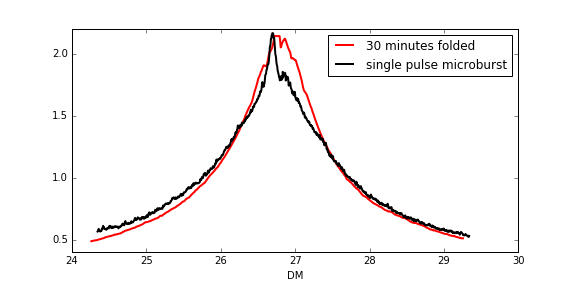
\includegraphics[trim={0.in 0in 0.in 0in}, width=\textwidth]{./figures/microstructure/DM_from_folded_pulse.png}
% \vspace{0.0cm}
% \caption{}
% \label{fig-micro}
% \end{center}
% \end{figure}



\section{Conclusion}
\label{sec:conclusion}
  
We have presented analysis of the largest collection 
of single-pulse microstructure data of 
B0329+54. Broadband microstructure was found to be a 
generic property of this pulsar, although it is
rarely highly modulated. The sub-pulses we analyzed often 
exhibited quasi-periodic trains of micropulses. We 
quantified such periodicity with a reduced autocorrelation 
function, which pulls out time-like correlations by 
first removing the stronger, smooth component of the 
sub-pulse. The quasi-periodic microstructure of B0329+54
were found to have no characteristic timescale, which is
different from other pulsars that have been studied. 
However, we did show that the range of periods are 
consistent with the known $T_\mu \approx 10^{-3}\,P$ relation. 
The micropulse widths are also roughly consistent with 
the known $t_\mu-P$ scaling. These scalings held for 
the polarized microstructure as well. Linear polarization 
and Stokes V were both found to mimic total intensity in 
their quasi-periodicities. As \citet{2015ApJ...806..236M} 
have shown, one would not necessarily expect this 
if the microstructure came from 
coherent curvature radiation of charged bunches.

The microburst widths allow us to estimate the Lorentz 
factor of the radiating particles, assuming the widths 
are due to relativistic beaming. We find $\gamma\sim200-1000$, 
which are inconsistent with the expected velocities. 
This inconsistency was also found by \citet{1998A&A...332..111L}, 
who use it to reject the beaming model. The other standard 
explanation for the origin of pulsar microstructure is not 
geometric but temporal. The idea is that time-like 
fluctuations in the magnetospheric plasma generate the 
periodic and quasi-periodic trains of sub-millisecond pulses
that are observed in a number of sources. 

In the framework of this model, we found the spectral 
behaviour of B0329+54's microstructure to be difficult
to interpret. In several strong pulses we found 
micropulses within a single sub-pulse to have very different 
broad-band frequency characteristics. If the pulses 
do not come from physically separate collections of 
charges, then we would not expect vastly different 
spectral properties. 

